\chapter{Anwendung von Pfadplanungsalgorithmen}

Algorithmen zur Pfadplanung finden in verschiedenen Bereichen Anwendung. Reale Pfadplanungsszenarien, wie Navigation und Logistik, sind durch Graphen modellierbar, auf die Suchalgorithmen angewendet werden können \cite{Botea.2011}. In Computerspielen werden Pfadplanungsalgorithmen für die Bewegung computergesteuerter Charaktere genutzt. Meist ist es von Interesse in kurzer Zeit ein angenähertes Ergebnis zu finden, damit der Spieler nicht lange warten muss \cite{Krishnaswamy.2009}. Dieses Gebiet birgt die zusätzliche Herausforderung die Bewegungen der Charaktere realistisch zu simulieren. Auch hat der Computer direkten Zugriff auf Umgebungsinformationen, sodass Schätzungen deutlich präziser vorgenommen werden können.


\section{Vergleich von BFS, Dijkstra und A*}

Der A* Algorithmus wird in vielen Videospielen für die Bewegungskontrolle von Nicht-Spieler Charakteren (engl. non-player character, NPC) genutzt \cite{Stamford.2014}. Der Grund dafür ist die in vielen Fällen schnellere Berechnung des kürzesten Pfads gegenüber uninformierten Algorithmen. In Abbildung 1 werden die Rechenzeiten der Algorithmen BFS, Dijkstra und A* in verschieden großen, quadratischen Umgebungen verglichen.


\begin{figure}[h]
	\centering
	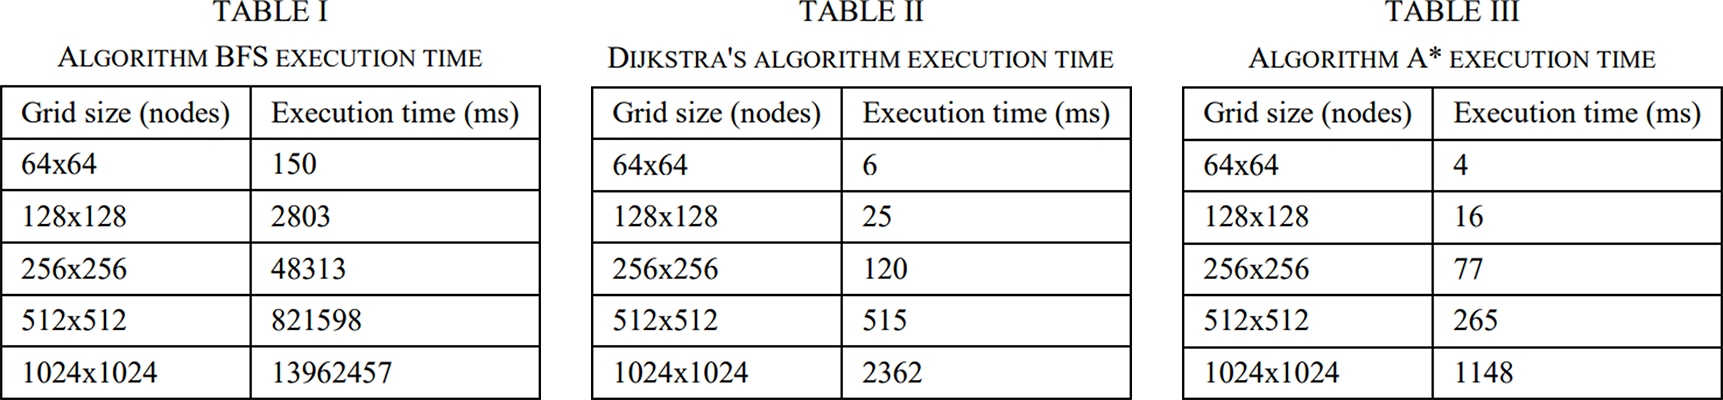
\includegraphics{images/Tables}
	\caption{in Anlehnung an}
	\label{fig:meine-grafik}
\end{figure}


\section{Erweiterung von A*}
Das Problem der Pfadplanung in Computerspielen muss in Echtzeit gelöst werden, und  häufig unter Einschränkungen des begrenzten Speichers und der begrenzten CPU-Ressourcen. Der Rechenaufwand, der erforderlich ist, um einen Pfad unter Verwendung eines Suchalgorithmus wie A * zu finden, nimmt mit der Größe des Suchraums zu. Daher kann die Pfadfindung auf großen Karten zu schwerwiegenden Leistungsengpässen führen. Daher kann das Reduzieren des Suchraums A * erheblich beschleunigen. Einer Erweiterung von A*-Algorithmus ist HPA*, welcher A* durch Reduzierung des Suchraums optimiert\cite{hpa}. %todo noch besser umschreiben

\subsection{Hierarchical Path-Finding A*}
Dies ist ein domänenunabhängiger Ansatz. Die Hierarchie kann auf mehr als zwei Ebenen erweitert werden, wodurch sie für große Problembereiche skalierbarer wird. Es wird ein dreistufiger Prozess angewendet. Der erste Schritt besteht darin, zur Grenze der Nachbarschaft zu fahren, die den Startort enthält. Der zweite Schritt besteht dann darin, nach einem Pfad von der Grenze der Startumgebung zur Grenze der Zielumgebung zu suchen. Dieser Schritt erfolgt auf abstrakter Ebene, wo die Suche einfacher und schneller ist. Der letzte Schritt besteht darin, den Pfad zu vervollständigen, indem Sie von der Grenze der Zielumgebung zur Zielposition fahren. HPA * hat bewiesen, dass es zehnmal schneller ist als A*\cite{hpa}

HPA* Verbesserungen
HPA kann auch verbessert werden. Path smoothing, Lazy Edge weight,

HPA* Anwendung%
HPA * ist gut für Videospiele geeignet, aber sehr allgemein. In der Praxis kann es sowohl für statische Welten, in denen die Graphhierarchie besser vorbereitet werden kann, erheblich optimiert werden, als auch in typischen dynamischen Welten, um häufige Geländeänderungen zu bewältigen. 
SHPA, 
DHPA



\section{Multi-Agent Pathfinding}
Ein Szenario in dem mehrere Akteure einen Pfad finden müssen, bei dem keine Kollisionen auftreten dürfen, bezeichnet man als Multi-Agent Pathfinding-Problem (MAPF). Es gibt verschiedene MAPF-Algorithmen, darunter Windowed Hierarchical Cooperative A*, Flow Annotated Replanning und Bounded Multi-Agent A*.

\subsection{Windowed Hierarchical Cooperative A*}
Bei dem Cooperative A*-Algorithmus sucht jeder Agent mit dem A*-Algorithmus in einem dreidimensionalen Graphen, um sein Ziel zu erreichen. Das Ergebnis der Suche teilt er mit den anderen Agenten in einer Reservierungstabelle. Auf diese Weise sind die Agenten in der Lage Kollisionen zu vermeiden. Der Hirarchical Cooperative A*-Algorithmus benutzt eine hierarchische Suche. Windowed Hierarchical Cooperative A*(WHCA*) begrenzt die Suchtiefe für jeden Agent zu einem Fenster. Sobald der Teilpfad in dem Fenster gefunden wurde folgt der Agent diesem Pfad und fängt mit der Berechnung des nächsten Teilpfades an. 
\subsection{Flow Annotated Replanning}
Ähnlich WHCA* nimmt Flow Annotation Replanning (FAR) die Pläne anderer Agentin in die Berechnung auf. Statt aber, wenn ein Pfad blockiert ist, einen neuen Pfad zu berechnen, wartet ein Agent im FAR-Algorithmus einfach auf dem aktuellen Knoten darauf, dass sein Pfad wieder frei wird und er ihn für sich reservieren kann. 

\subsection{Bounded Multi-Agent A*}
Bounded Mulit-Agent A* basiert auf Real-time Adaptive A*(RTAA*). RTAA* wird für ein Multiagenten-Setting erweitert. Andere Agenten werden während der Suche als sich bewegende Hindernisse betrachtet. AUßerdem haben Agenten die Möglichkeit andere Agenten dazu aufzufordern Zellen frei zu machen. Der aufgeforderte Agent wird zu einer freien benachbarten Zelle wandern und seine reguläre Such von dort aus fortführen\cite{Sigurdson.2019}.


\section{Verwandte Arbeiten} 
Pfadplanungsproblem wird oft ebenfalls in Robotik untersucht. Eine Abbildung der realen Welt muss deren Merkmale möglichst präzis erfassen können. In \cite{lozano} und \cite{latombe} wird einer Konfigurationsraum beschrieben. Die Idee besteht darin, dass ein Roboter als ein Punkt betractet wird. Nach Latombe\cite{latombe}, es existieren folgende Ansätze für Pfadpalnung in einem Konfigurationsraum: Wegkartenverfahren, Zellunterteilungsverfahren und Potentialfelderverfahren. 


Bei \textbf{Wegkartenverfahren} wird der Konfigurationsraum in Kurven unterteilt. Einige Versionen davon sind z.B Voronoi-Diagramm\cite{voronoi} und der Sichtbarkeitsgraph\cite{visG1}. Das \textbf{Potentialfeldverfahren} bietet einen Ansatz, bei dem der Suchraum von Gradienten überspannt wird. Aus den Gradienten werden dann mögliche Bewegungsrichtungen ersichtlich. Die \textbf{Zellzerlegung}\cite{cd} ist ein bekanntes Hindernisvermeidungsverfahren, das den hindernisfreien Konfigurationsraum in eine endliche Sammlung nicht überlappender(disjunkter) konvexer Polygone, sogenannte Zellen, zerlegt. In diesen kann leicht ein Pfad gefunden werden.
